%%%% Dokumentklassen %%%%

\documentclass[a4paper,11pt,fleqn,dvipsnames,twoside,openright]{memoir} 	% Openright åbner kapitler på højresider (openany begge)


%%%% PACKAGES %%%%

%% Oversættelse og tegnsætning %%
\usepackage[utf8]{inputenc}					% Input-indkodning af tegnsæt (UTF8)
\usepackage[danish]{babel}					% Dokumentets sprog
\usepackage[T1]{fontenc}					    % Output-indkodning af tegnsæt (T1)
\usepackage{ragged2e,anyfontsize}			% Justering af elementer
\usepackage{fixltx2e}						% Retter forskellige fejl i LaTeX-kernen
																			
%% Figurer og tabeller (floats) %%
\usepackage{graphicx} 						% Håndtering af eksterne billeder (JPG, PNG, EPS, PDF)
\usepackage{multicol}         	            	% Muliggør output i spalter
\usepackage{rotating}						% Rotation af tekst med \begin{sideways}...\end{sideways}
\usepackage{xcolor}							% Definer farver med \definecolor. Se mere: http://en.wikibooks.org/wiki/LaTeX/Colors
\usepackage{flafter}						% Sørger for at floats ikke optræder i teksten før deres reference
\let\newfloat\relax 						% Justering mellem float-pakken og memoir
\usepackage{float}							% Muliggør eksakt placering af floats, f.eks. \begin{figure}[H]

%% Matematik mm. %%
\usepackage{amsmath,amssymb,stmaryrd} 		% Avancerede matematik-udvidelser
\usepackage{mathtools}						% Andre matematik- og tegnudvidelser
\usepackage{textcomp}                 		% Symbol-udvidelser (fx promille-tegn med \textperthousand)
\usepackage{rsphrase}						% Kemi-pakke til RS-saetninger, fx \rsphrase{R1}
\usepackage[version=3]{mhchem} 				% Kemi-pakke til flot og let notation af formler, f.eks. \ce{Fe2O3}
\usepackage{siunitx}						% Flot og konsistent præsentation af tal og enheder med \si{enhed} og \SI{tal}{enhed}
\sisetup{output-decimal-marker = {,}}		% Opsætning af \SI (DE for komma som decimalseparator) 

%% Referencer og kilder %%
\usepackage[danish]{varioref}				% Muliggør bl.a. krydshenvisninger med sidetal (\vref)
\usepackage{natbib}							% Udvidelse med naturvidenskabelige citationsmodeller
\usepackage{xr}							    % Referencer til eksternt dokument med \externaldocument{<NAVN>}

%% Misc. %%
\usepackage{listings}						% Placer kildekode i dokumentet med \begin{lstlisting}...\end{lstlisting}
\usepackage{lipsum}							% Dummy text \lipsum[..]
\usepackage[shortlabels]{enumitem}			% Muliggør enkelt konfiguration af lister
\usepackage{pdfpages}						% Gør det muligt at inkludere pdf-dokumenter med kommandoen \includepdf[pages={x-y}]{fil.pdf}	
\pdfoptionpdfminorversion=6					% Muliggør inkludering af pdf-dokumenter, af version 1.6 og højere
\pretolerance=2500 							% Justering af afstand mellem ord (højt tal, mindre orddeling og mere luft mellem ord)	


%%%% CUSTOM SETTINGS %%%%

%% Marginer %%
\setlrmarginsandblock{3.5cm}{2.5cm}{*}		% \setlrmarginsandblock{Indbinding}{Kant}{Ratio}
\setulmarginsandblock{2.5cm}{3.0cm}{*}		% \setulmarginsandblock{Top}{Bund}{Ratio}
\checkandfixthelayout 						% Oversætter værdier til brug for andre pakker

%% Afsnitsformatering %%
\setlength{\parindent}{0mm}           		% Størrelse af indryk
\setlength{\parskip}{3mm}          			% Afstand mellem afsnit ved brug af double Enter
\linespread{1,1}							% Linjeafstand

%% Indholdsfortegnelse %%
\setsecnumdepth{subsection}		 			% Dybden af nummererede overskrifter (part/chapter/section/subsection)
\maxsecnumdepth{subsection}					% Dokumentklassens grænse for nummereringsdybde
\settocdepth{subsection} 					% Dybden af indholdsfortegnelsen
		
%% Opsætning af listings %%
\definecolor{commentGreen}{RGB}{34,139,24}
\definecolor{stringPurple}{RGB}{208,76,239}

\lstset{language=Matlab,					    % Sprog
	basicstyle=\ttfamily\scriptsize,		    % Opsætning af teksten
	keywords={for,if,while,else,elseif,		% Nøgleord at fremhæve
			  end,break,return,case,
			  switch,function},
	keywordstyle=\color{blue},				% Opsætning af nøgleord
	commentstyle=\color{commentGreen},		% Opsætning af kommentarer
	stringstyle=\color{stringPurple},		% Opsætning af strenge
	showstringspaces=false,					% Mellemrum i strenge enten vist eller blanke
	numbers=left, numberstyle=\tiny,		    % Linjenumre
	extendedchars=true, 					    % Tillader specielle karakterer
	columns=flexible,						% Kolonnejustering
	breaklines, breakatwhitespace=true,		% Bryd lange linjer
}

%% Navngivning %%
\addto\captionsdanish{
	\renewcommand\appendixname{Appendiks}
	\renewcommand\contentsname{Indholdsfortegnelse}	
	\renewcommand\appendixpagename{Appendiks}
	\renewcommand\appendixtocname{Appendiks}
	\renewcommand\cftchaptername{\chaptername~}		% Skriver "Kapitel" foran kapitlerne i indholdsfortegnelsen
	\renewcommand\cftappendixname{\appendixname~}	% Skriver "Appendiks" foran appendiks i indholdsfortegnelsen
}

%% Kapiteludssende %%
\definecolor{numbercolor}{gray}{0.7}		            % Definerer en farve til brug til kapiteludseende
\newif\ifchapternonum

\makechapterstyle{jenor}{					        % Definerer kapiteludseende frem til ...
  \renewcommand\beforechapskip{0pt}
  \renewcommand\printchaptername{}
  \renewcommand\printchapternum{}
  \renewcommand\printchapternonum{\chapternonumtrue}
  \renewcommand\chaptitlefont{\fontfamily{pbk}\fontseries{db}\fontshape{n}\fontsize{25}{35}\selectfont\raggedleft}
  \renewcommand\chapnumfont{\fontfamily{pbk}\fontseries{m}\fontshape{n}\fontsize{1in}{0in}\selectfont\color{numbercolor}}
  \renewcommand\printchaptertitle[1]{%
    \noindent
    \ifchapternonum
    \begin{tabularx}{\textwidth}{X}
    {\let\\\newline\chaptitlefont ##1\par} 
    \end{tabularx}
    \par\vskip-2.5mm\hrule
    \else
    \begin{tabularx}{\textwidth}{Xl}
    {\parbox[b]{\linewidth}{\chaptitlefont ##1}} & \raisebox{-15pt}{\chapnumfont \thechapter}
    \end{tabularx}
    \par\vskip2mm\hrule
    \fi
  }
}											        % ... her

\chapterstyle{jenor}						        % Valg af kapiteludseende - Google 'memoir chapter styles' for alternativer

%% Sidehoved %%

\makepagestyle{AAU}							        % Definerer sidehoved og sidefod udseende frem til ...
\makepsmarks{AAU}{%
	\createmark{chapter}{left}{shownumber}{}{. \ }
	\createmark{section}{right}{shownumber}{}{. \ }
	\createplainmark{toc}{both}{\contentsname}
	\createplainmark{lof}{both}{\listfigurename}
	\createplainmark{lot}{both}{\listtablename}
	\createplainmark{bib}{both}{\bibname}
	\createplainmark{index}{both}{\indexname}
	\createplainmark{glossary}{both}{\glossaryname}
}
\nouppercaseheads									% Ingen Caps ønskes

\makeevenhead{AAU}{\small ST2PRJ2 Gruppe 1}{}{\leftmark}	% Definerer lige siders sidehoved (\makeevenhead{Navn}{Venstre}{Center}{Hoejre})
\makeoddhead{AAU}{\rightmark}{}{\small ASE}		            % Definerer ulige siders sidehoved (\makeoddhead{Navn}{Venstre}{Center}{Højre})
\makeevenfoot{AAU}{\small \thepage}{}{}						% Definerer lige siders sidefod (\makeevenfoot{Navn}{Venstre}{Center}{Højre})
\makeoddfoot{AAU}{}{}{\small \thepage}						% Definerer ulige siders sidefod (\makeoddfoot{Navn}{Venstre}{Center}{Højre})

\copypagestyle{AAUchap}{AAU}							% Sidehoved for kapitelsider defineres som standardsider, men med blank sidehoved
\makeoddhead{AAUchap}{}{}{}
\makeevenhead{AAUchap}{}{}{}
\makeheadrule{AAUchap}{\textwidth}{0pt}
\aliaspagestyle{chapter}{AAUchap}					% Den ny style vælges til at gælde for chapters
													% ... her
															
\pagestyle{AAU}										% Valg af sidehoved og sidefod


%%%% CUSTOM COMMANDS %%%%

%% Billede hack %%
\newcommand{\figur}[4]{
		\begin{figure}[H] \centering
			\includegraphics[width=#1\textwidth]{billeder/#2}
			\caption{#3}\label{#4}
		\end{figure} 
}

%% Specielle tegn %%
\newcommand{\decC}{^{\circ}\text{C}}
\newcommand{\dec}{^{\circ}}
\newcommand{\m}{\cdot}


%%%% ORDDELING %%%%

\hyphenation{}


%%%% Tilføjelser af min preample %%%%

% Booktabs:
% The booktabs package is needed for better looking tables. 
\usepackage{booktabs}

% Caption:
% For better looking captions. See caption documentation on how to change the format of the captions.
\usepackage[hang, font={small, it}]{caption}

% Hyperref:
% This package makes all references within your document clickable. By default, these references will become boxed and colored. This is turned back to normal with the \hypersetup command below.
\usepackage{hyperref}
	\hypersetup{colorlinks=false,pdfborder=0 0 0}

% Cleveref:
% This package automatically detects the type of reference (equation, table, etc.) when the \cref{} command is used. It then adds a word in front of the reference, i.e. Fig. in front of a reference to a figure. With the \crefname{}{}{} command, these words may be changed.
\usepackage{cleveref}
	\crefname{equation}{formel}{formler}
	\crefname{figure}{figur}{figurer}	
	\crefname{table}{tabel}{tabeller}

% Mine tilføjelser:
\usepackage{units}                        %% Bruges til at gøre fx 1/2 samlet med: \nicefrac{1}{2}.
\usepackage{tabu, longtable}              %% Bruges til tabeller.
\setlength{\tabulinesep}{1.5ex}           %% Definerer linjeafstand i tabeller.
\usepackage{enumerate}                    %% Bruges til lister.
\usepackage{tabto}                        %% Giver mulighed for TAB med fx \tabto{3em}.
\usepackage[hyphenbreaks]{breakurl}       %% Bruges til websiders url'er.
\renewcommand{\UrlFont}{                  %% Definerer url-font.
\small\ttfamily}                          %
\bibliographystyle{plain}                 %% Definere bibliografien. Ses til sidst i dokumentet i kapitlet Litteratur.
\raggedbottom

%\externaldocument[D-]{Dokumentation}

\begin{document}	
\frontmatter						% Nummereres med romerske tal.
\begin{titlingpage}
\begin{center}

~ \\[3cm]


\includegraphics[width=0.6\textwidth]{figurer/ASE.png}~\\[1cm]

\textsc{\LARGE Aarhus School of Engineering}\\[1.5cm]

\textsc{\Large Sundhedsteknologi}\\
\textsc{\Large 2. semesterprojekt}\\[0.5cm]

\noindent\makebox[\linewidth]{\rule{\textwidth}{0.4pt}}\\
[0.5cm]{\Huge Rapport}
\noindent\makebox[\linewidth]{\rule{\textwidth}{0.4pt}}

\end{center}

\textit{Gruppe 1} \newline
Lise Skytte Brodersen (201407432) \newline
Mads Fryland J\o rgensen (201403827) \newline
Albert Jakob Fredshavn (201480425) \newline
Malene Cecilie Mikkelsen (201405722) \newline		 
Mohamed Hussein Mohamed (201370525) \newline 
Sara-Sofie Staub Kirkeby (201406211) \newline
Martin Banasik (201408398) \newline
Cecilie Ammizb\o ll Aar\o e (201208778) \newline 


\textit{Vejleder} \newline
Studentervejleder\\
Lars Mortensen\\
Aarhus Universitet\\
\pageref{LastPage}



\vfill

\begin{center}
{\large \today}
\end{center}


\end{titlingpage}
\chapter{Resumé}
\begin{vplace}[0.6]
{\large \textit{Gruppemedlemmer}}
\\
\\

\noindent \begin{tabular}{ll}
	\makebox[3.0in]{\hrulefill} & \makebox[1.5in]{\hrulefill}\\
	Lise Skytte Brodersen (201407432) & Dato\\[7ex]% adds space between the two sets of signatures
	\makebox[3in]{\hrulefill} & \makebox[1.5in]{\hrulefill}\\
	Mads Fryland J\o rgersen (201403827) & Dato\\[7ex]
	\makebox[3in]{\hrulefill} & \makebox[1.5in]{\hrulefill}\\
	Albert Jakob Fredshavn (201408425) & Dato\\[7ex]
	\makebox[3in]{\hrulefill} & \makebox[1.5in]{\hrulefill}\\
	Malene Cecilie Mikkelsen (201405722) & Dato\\[7ex]
	\makebox[3in]{\hrulefill} & \makebox[1.5in]{\hrulefill}\\
	Mohamed Hussein Mohamed (201370525) & Dato\\[7ex]
	\makebox[3in]{\hrulefill} & \makebox[1.5in]{\hrulefill}\\
	Sara-sofie Staub Kirkeby (201406211) & Dato\\[7ex]
	\makebox[3in]{\hrulefill} & \makebox[1.5in]{\hrulefill}\\
	Martin Banasik (201408398) & Dato\\[7ex]
	\makebox[3in]{\hrulefill} & \makebox[1.5in]{\hrulefill}\\
	Cecilie Ammitzb\o ll Aar\o e (201208778) & Dato\\[7ex]
	
\end{tabular}
\\
{\large \textit{Vejleder}}
\\
\\
\\
\noindent \begin{tabular}{ll}
	\makebox[3.0in]{\hrulefill} & \makebox[1.5in]{\hrulefill}\\
	Lars Mortensen & Dato\\[8ex]
\end{tabular}
\end{vplace}

\chapter{Godkendelsesformular}

{\LARGE\textit{Godkendelsesformular}}

{\large Forfattere:}
\\[5ex]


\begin{tabular}{c c}
\centering 
	\makebox[2.0in]{\hrulefill} & \makebox[2.0in]{\hrulefill}\\
	Lise Skytte Brodersen & Mads Fryland Jørgensen\\[7ex]
	\makebox[2.0in]{\hrulefill} & \makebox[2.0in]{\hrulefill}\\
	Albert Jakob Fredshavn & Malene Cecilie Mikkelsen\\[7ex]
	\makebox[2.0in]{\hrulefill} & \makebox[2.0in]{\hrulefill}\\
	Mohamed Hussein Mohamed & Sara-Sofie Staub Kirkeby\\[7ex]
	\makebox[2.0in]{\hrulefill} & \makebox[2.0in]{\hrulefill}\\
	Martin Banasik & Cecilie Ammitzøll Aarøe\\[7ex]

\end{tabular}

\begin{tabular}{c c c c}
	\textbf{Godkendes af:} & Lars Mortensen\\[3ex]
	\textbf{Antal sider} & <antalsider>\\[3ex]
	\textbf{Kunde} & Aarhus Universitet
\end{tabular}\\[8ex]
Ved underskrivelse af dette dokument accepteres det af begge parter som værende kravene til udviklingen af det ønskede system.
\\
\\
\textbf{Dato: } 28/5-2015\\[7ex]

\begin{tabular}{c c}
	\makebox[2.0in]{\hrulefill} & \makebox[2.0in]{\hrulefill}\\
	\centering 
	Kundens underskrift & Leverandørens underskrift
\end{tabular}

\chapter{Ordliste}

\begin{longtabu} to \linewidth{@{}l X[j]@{}}
    Ord &    Forklaring\\
    \toprule 
	EKG	&	Elektrokardiografi\\
	DAQ	&	Data acquisition\\
	AV-klapper	&	Atrioventrikulær-klapperne\\
	AV-knuden	&	Atrioventrikulær-knuden\\
	ISE & Indledende System Engineering \\
	SysML & System Modeling Language \\
	BDD & Block Defination Diagram \\
	IBD & Intern Block Diagram\\
	SD & Sekvensdiagram\\
	UML & Unified Modeling Language\\
	Cerebral apopleksiske &	Slagtilfælde i hjernen (blodprop/hjerneblødning)\\
	Hjerteinsufficiens	&	Hjertesvigt\\
\label{forkort}
\end{longtabu}
\cleardoublepage		

\tableofcontents*                   % Indsætter en indholdsfortegnelse før Indledning.

\mainmatter                         % Her findes de nummererede kapitler modsat \frontmatter og \backmatter. Nummereres med arabiske tal.
\subsubsection{Versionhistorik}

\begin{longtabu} to \linewidth{@{}l l l X[j]@{}}
    Version &    Dato &    Ansvarlig &    Beskrivelse\\[-1ex]
    \midrule
    Tekst &    Tekst &    Tekst &    Tekst.\\
\label{version_Systemark}
\end{longtabu}

\chapter{Indledning}
I dagens Danmark er incidensen af hjertesygdomme på ca. 45.000 nye tilfælde årligt\footnote{http://www.si-folkesundhed.dk/upload/hjertekarsygdomme\_i\_2011-2\_rapport.pdf}. Mange typer af hjertesygdomme diagnosticeres via et EKG-apparat, der måler patientens hjerteimpulser. Disse impulser bliver afbildet som en graf, der indeholder P-, Q-, R-, S- og T-takker. Det er forholdet mellem disse takker, der fortæller, hvordan hjerteimpulserne hos patienten er. Hvis en patient har et rask EKG-signal, skal forholdet mellem takkerne være indenfor nogle bestemte intervaller. Et EKG-signal, der afviger fra disse standarter siges at være abnormalt og patienten bør tjekkes for en eventuel hjertesygdom. Derfor er et EKG-apparat en vigtig teknologi indenfor sundhedsvæsenet i forhold til videre diagnosticering af hjertesygdomme.\\ \\
Formålet med dette projekt er, at udvikle en software, som netop har til formål at detektere en selvvalgt hjertesygdom. Den nødvendige hardware samt et stykke kode, der betragtes som Blackbox, er blevet udleveret ved projektets start.\\
Dette specifikke projekt omhandler sygdommen atrieflimren. En sygdom, der særligt omfatter den ældre befolkning, da prævalensen i Danmark er 5-10\%\footnote{https://www.sundhed.dk/borger/sygdomme-a-aa/hjerte-og-blodkar/sygdomme/hjertearytmier/atrieflimren-og-flagren/} for borgere over 80 år.\\
Atrieflimren forekommer, når patientens atrie-kontraktionsmønster forstyrres og dermed begynder at flimre. Atrieflimren karakteriseres ved, at der forekommer 220-300 små udsving pr. minut på EKG-signalets baseline. Desuden vil der i frekvensspektret 300-400 Hz, opstå forhøjede amplituder. Det er ud fra denne karakteristik af amplituder, der, i Visual Studio, er blevet udarbejdet en analyse, som kan detektere atrieflimren. Denne analyse er en del af et større program, hvis formål også er, at kunne visualisere og gemme et et givet EKG-signal i en privat- samt offentlig database. \\ \\
Rapporten er udført som en naturvidenskabelig rapport med først og fremmest et baggrundsafsnit. Dette afsnit fortæller overordnet omkring hjertets funktionalitet, atrieflimren og elektrokardiografi. Det er denne teori, som ligger til grund for systemets design og opbygning, samt hvilke krav, der er stillet til systemet.
  

\chapter{Projektformulering}
\section{Problemformulering}
 I dette projekt vil vi udvikle en software, som ud fra en virtuel patients EKG-målinger kan detektere atrieflimmer. 
\section{Indledning}
Via kendskabet til raske EGK-signaler, ved vi hvordan forholdet mellem P-, Q-, R-, S- og T-takkerne normalt er. Ud fra dette kan vi programmere et system, som kan analysere et givet abnormalt EKG-signal, og dermed informere brugeren fx i form af sundhedsfagligt personale om eventuelle forekomster af atrieflimmer.\\
Udover at detektere og informere om atrieflimmer kan softwaren også danne en graf og gemme de givne data i en SQL-database. Softwaren er opbygget via trelagsmodellen, som består af et data-, logik- og GUI-lag.
\\
Det abnormale EKG-signal hentes ned i form af en csv-fil fra den eksterne EKG-database, Physionet (lav reference eller ordliste). Csv-filens data omdannes via Analog-discovery til et analogt signal. Det analoge signal omdannes via DAQ'en til et digitalt signal. Det er dette digitale signal softwaren behandler, og er dermed det signal, der dannes en graf ud fra. Softwaren detekterer atrieflimmer og informerer brugeren herom.     


1. rask hjerte\\
2. EKG-signaler generelt inkl. beskrivelse af takker\\
3. patofysiologi - atrieflimmer inkl. detektion via EKG\\
4. Software og hardware beskrivelse
\chapter{Baggrund}

\section{Hjertet}
Hjertet, \textit{cor}, er en hul muskel, der har til opgave at pumpe blodet rundt til hele kroppen. Hjertet består af i alt fire kamre, som det kan ses på figur 3.1 nedenfor. To forkamre, atrier, og to hjertekamre, ventrikler. Atrierne fungere primært som reservoir for blod, mens ventriklerne fungerer som den effektive pumpe.\\

\begin{figure}[htb]
	\centering
	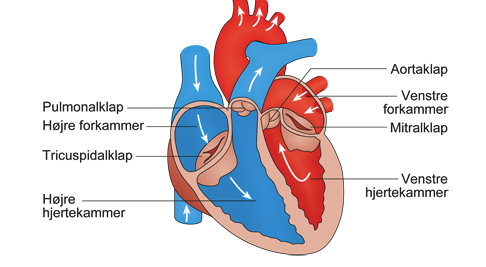
\includegraphics[width=1\textwidth]{Figurer/Snip20150410_31}
	\caption{Hjerte med forklarende pile \protect\footnotemark} 
\end{figure}
\footnotetext{http://www.hjertelunge.dk/hjertesygdomme/hjerte\_og\_kredsloeb/hjertet/}

Hjertekamrene og forkamrene er adskilt fra hinanden af anulus fibrosus, som er en plade af bindevæv. Anulus fibrosus består af fire bindevævsringe, der er forbundet med hinanden. To af disse udgør åbningerne mellem atrierne og ventriklerne. De to sidste danner åbningerne mellem højre hjertekammer og lungepulsåren og venstre ventrikel og hovedpulsåren. Ved alle bindevævsringene er der klapper, der fungere som ventiler.\\ 
AV-klapperne sidder mellem atrierne og ventriklerne. Klappen mellem højre atrium og ventrikel kaldes tricuspidalklap, mens klappen mellem venstre atrium og ventrikel kaldes mitralklap, se figur 3.1. Aortaklappen er placeret ved afgangen af hovedpulsåren og pulmonalklappen ved afgangen af lungepulsåren. Klapperne fungere således, at blodet kun kan løbe én vej gennem dem. Åbningen samt lukningen af disse er en passiv proces, som bestemmes af forskelle i væsketrykket på de to sider af klapperne.\\ 

\begin{figure}[htb]
	\centering
	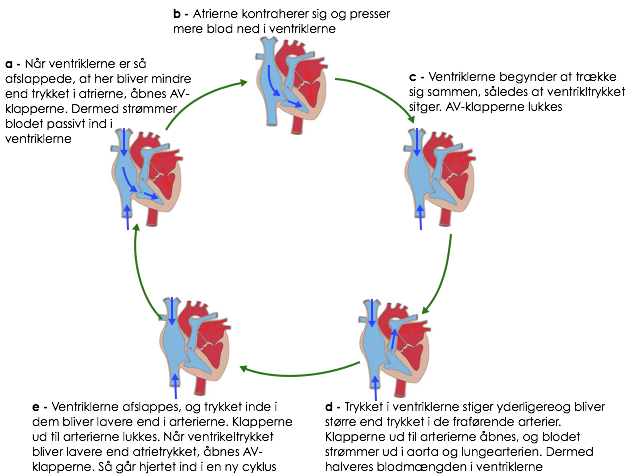
\includegraphics[width=1\textwidth]{Figurer/Snip20150412_7}
	\caption{De forskellige faser i hjertets cyklus \protect\footnotemark}
\end{figure}
\footnotetext{Billede fra "Menneskets anatomi og fysiologi" s. 273 figur 9.6}

Hjertets cyklus, som er illustreret ved figur 3.2, inddeles i to hovedfaser. Den første kaldes diastolen. I diastolen er ventriklerne afslappede og fyldes med blod. Det vil sige, at trykket i ventriklerne bliver lavere end trykket i atrierne, således at AV-klapperne åbnes, og blodet begynder at strømme ind i ventriklerne. Under hele diastolen er aortaklappen lukket. Den anden fase kaldes systolen. I systolen kontraherer ventriklerne sig. Trykket i ventriklerne overstiger trykket i atrierne således, at AV-klapperne lukkes, så tilbagestrømning af blod til atrierne forhindres. Når ventriklerne har kontraheret sig så meget, at trykket i ventriklerne overstiger trykket i hovedpulsåren samt i lungepulsåren, åbnes aortaklappen og pulmonalklappen, og blodet strømmer ud i hovedpulsåren og lungepulsåren. Ventriklernes tryk falder igen til under atriernes tryk, hvilket påvirker, at AV-klapperne åbnes igen og hjertets cyklus starter forfra.\\
Hjertets cyklus igangsættes i sinusknuden ved aktionspotentialer, der føres til de forskellige dele af hjertet. Dette sker enten ved, at aktionspotentialet går fra hjertemuskelcelle til hjertemuskelcelle gennem åbne celleforbindelser, eller gennem åbne celleforbindelser mellem specialiserede hjertemuskelceller i hjertets specielle ledningssystem. Det specielle ledningssystem består af tre sammenhængende dele - AV-knuden, det hiske bundt gennem anulus fibrosus og det hiske bundt over i purkinjefibrene(se figur 3.3). \\
Hjertets ledningssystem har to hovedopgaver. Først at sørge for, at aktionspotentialet spredes hurtigt gennem hjertet, og dermed sørge for al hjertemuskulaturen i ventriklen kontraheres næsten samtidig. Denne næsten samtidige kontraktion medfører, at der inde i ventriklerne opbygges et effektivt tryk. Purkinjefibrene, som kun er i ventriklerne og ikke atrierne, gør at aktionspotentialerne spredes hurtigere i ventriklerne end i atrierne. Den anden hovedopgave er derfor at sikre en vis forsinkelse i impulsledning fra atrierne til ventriklerne. Forsinkelsen er mulig, da anulus fibrosus fungerer som en elektrisk isolator. Derfor skal aktionspotentialet ledes fra atrierne til ventriklerne via det specialiserede ledningssystem, og da AV-knuden leder aktionspotentialet særlig langsomt, opstår forsinkelsen. Dette medfører, at atriernes kontraktion fuldføres, før ventriklernes igangsættes, dermed er der sikret en tilstrækkelig fyldning af ventriklerne, før de pumper blodet videre. Denne spredning og udløsning af aktionspotentiale sker regelmæssigt, og er den afgørende faktor for hjertets kontraktions rytme.
\begin{figure}[htb]

	\centering	
	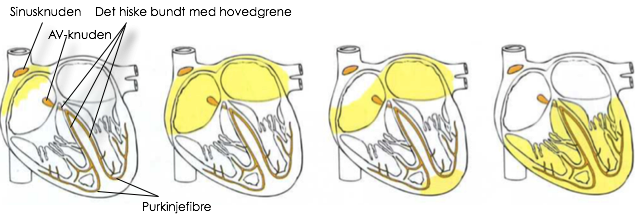
\includegraphics[width=1\textwidth]{Figurer/Snip20150410_6}
	\caption{Spredning af aktionspotentialer gennem hjertet \protect\footnotemark}
\end{figure}
\footnotetext{"Menneskets anatomi og fysiologi" s. 275 figur 9.9}

I figur 3.3 ses spredningen af aktionspotentialer gennem hjertet. Aktionspotentialet udløses i sinusknuden og forsinkes i AV-knuden. Dernæst ledes aktionspotentialet videre til ventrikelmuskulaturen. De farvelagte områder er de depolariserede områder og det ses, at atriernes depolarisering er afsluttet før ventriklernes er startet.

\section{Elektrokardiogram}
Et elektrokardiogram, EKG, afspejler hjertets elektriske aktivitet. Teknikken kaldes elektrokardiografi og udføres via elektroder, der er placeret forskellige steder på kroppen, primært omkring hjertet. Elektroderne måler den elektriske aktivitet via en overfladespænding, der går ud fra thorax. Det er disse elektriske spændinger, som danner de forskellige graf-udsving, som er EKG-signalets takker. Takkerne viser atriernes- og ventriklernes systole og diastole, og er inddelt i P-takken, QRS-komplekset og T-takken. Grafisk vil EKG signalet være vist som det ses på figur 3.4 nedenfor.

\begin{figure}[H]
	\centering
	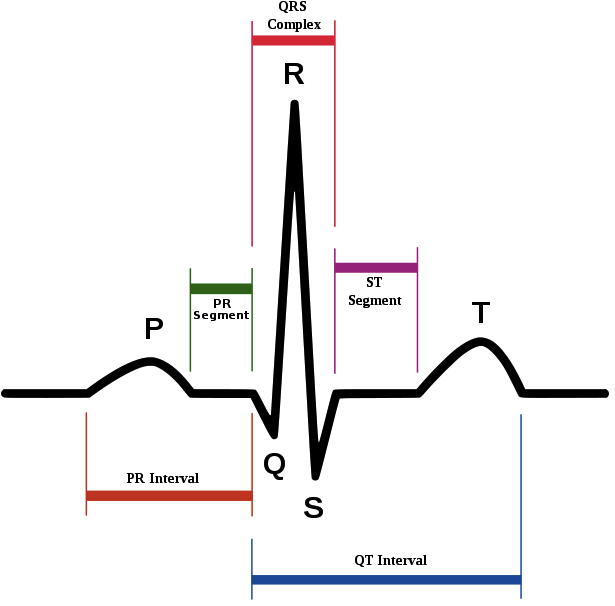
\includegraphics[width=0.7\textwidth]{Figurer/Snip20150412_36}
	\caption{Normalt EKG-signal \protect\footnotemark}
\end{figure}
\footnotetext{http://en.wikipedia.org/wiki/QRS\_complex\#/media/File:SinusRhythmLabels.svg}

P-takken viser atriets depolarisering. Dernæst kommer PR-segmentet, som er den forsinkede strøm fra atrier til ventrikler. QRS-komplekset udgør ventrikeldepolariseringen. QRS-komplekset er større end P-takken, da muskelmassen i ventriklerne er større end atriernes muskelmasse, hvilket påvirker en højere elektrisk aktivitet. T-takken beskriver ventriklernes repolarisering. Denne er også mindre end QRS-komplekset, da repolariseringen forløber langsommere end depolariseringen.\\
Elektrokardiografi giver et billede af, hvordan hjertet fungerer. På figur 3.4 ses et EKG-signal for et raskt hjerte. Ved et raskt hjerte vil intervallerne mellem takkerne i EKG-signalet være følgende: 

\begin{itemize}
	\item PR Interval: 0.12 - 0.20 sekunder
	\item QRS Complex: 0.08 - 0.10 sekunder 
	\item QT Interval: 0.4 - 0.43 sekunder 
	\item RR Interval: 0.6 - 1.0 sekunder 
\end{itemize}

 Hvis hjertet ikke fungere optimalt, vil EKG-signalet se anderledes ud, og en sundhedsfaglig person vil kunne diagnosticere eventuelle sygdomme ud fra grafen.  En patient kunne eventuelt have atrieflimren, som er den sygdom, dette projekt omhandler.  


\section{Atrieflimren}
Atrieflimren forekommer, når atrierne ikke kontraherer sig ordentligt. Den hyppigste udløsning af atrieflimren forefalder pga. en serie af hurtige impulser (ekstrasystoler), hvilket er illustreret på første del af figur 3.5.  Ekstrasystolerne kommer fra den atriemuskulatur, som sidder nær lungevenerne i venstre atrium. Dermed bliver atriernes normale kontraktionsmønster ødelagt, og de begynder at "flimre". Under atrieflimren fungerer sinusknuden stadig som normalt, men har ingen kontakt til atrium.\\
Pga. arytmien mister man den regelmæssige atrietømning og får nedsat funktion af hjertets pumpning. Blodet vil ophobe sig i atriet og danne lokale tromber.  De kan løsrive sig og flyde med blodstrømmen ud i kroppen, hvor de kan sætte sig fast (embolisere). Ubehandlet emboliserende atrieflimren er årsagen til 1/3 af alle cerebral apopleksiske tilfælde. Derfor er det vigtigt at være opmærksom på tilstedeværelse af atrieflimren hos netop disse patienter.\\
Hvis arytmien står på i længere tid, og ventrikelfrekvensen er hurtig, kan det udløse hjerteinsufficiens med tiltagende dilatation og dårlig kontraktion af ventriklerne. \\
Atrieflimren opstår som anfald (paroksystisk), der spontant konverterer tilbage til normal sinusrytme efter få timer til dage. Med årerne bliver arytmien mere vedvarende (persisterende) for til sidst at blive kronisk.  De symptomer, som kan forbindes med atrieflimren er en øget træthed, åndenød og en forhøjet samt uregelmæssig puls, der kan være utydelig og hurtig. Desuden vil blodtrykket falde, og der kan være tegn på hjerteinsufficiens, både i højre og venstre side af hjertet. 

\begin{figure}[htb]
	\centering
	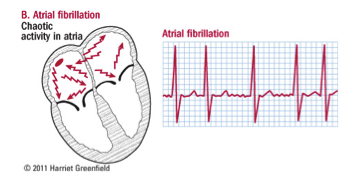
\includegraphics[width=1\textwidth]{Figurer/Snip20150412_32}
	\caption{Aktivitet i atrie ved atrieflimren\protect\footnotemark}
\end{figure}
\footnotetext{http://www.health.harvard.edu/heart-health/atrial-fibrillation-common-serious-treatable}

Diagnosen stilles via elektrokardiografi. EKG-grafen er domineret af mange irregulære og smalle QRS-komplekser uden ordentlige P-takker, som set på figur 3.5 ovenover. Med andre ord siges det, at der forekommer 220-300 små udsving/minut. Der kan også være forhøjede amplituder i frekvensspektret 300-400 Hz. Hvis disse forhold forekommer, kan patienten muligvis have atrieflimren.\\ 
Den hyppigste form for behandling er ved betablokkere, flekainid, dronaderon og amiodaron. Der indføres katere i venstre atrium, som ødelægger atriemuskulaturen, hvilket udløser flimren.

  

%\include{rfiler/Arbejdsmetoder}
%\include{rfiler/Resultater}
%\include{rfiler/Diskussion}
%\include{rfiler/Konklusion}
%\include{rfiler/Erfaringer}
%\include{rfiler/Udvikling}

\backmatter
%\include{rfiler/Bilagliste}

%\bibliography{bibliografi/PRJ3}    % Sætter bibliografien bagerst i dokumentet. Bruger bib-filen PRJ3.

\end{document}